\documentclass[final]{IEEEtran}
\usepackage[dvips]{graphicx}
\usepackage{amsmath,amssymb}
\usepackage{array}
\usepackage{diagbox}
\usepackage{url}
\usepackage{multirow}
\usepackage[utf8]{inputenc}
\usepackage{supertabular}
\usepackage{marvosym}
\usepackage[]{algorithm2e}
\usepackage{bbm}
\usepackage{tikz}
\usepackage{tikzscale}
\usepackage{pgf}
\usetikzlibrary{calc,decorations.pathreplacing,positioning,shadows,backgrounds,arrows.meta,shapes.geometric}
\DeclareUnicodeCharacter{20AC}{\EUR{}}

\SetKwInOut{Initialization}{Initialization}

\allowdisplaybreaks

% avoid overflowing urls
\expandafter\def\expandafter\UrlBreaks\expandafter{\UrlBreaks%  save the current one
  \do\a\do\b\do\c\do\d\do\e\do\f\do\g\do\h\do\i\do\j%
  \do\k\do\l\do\m\do\n\do\o\do\p\do\q\do\r\do\s\do\t%
  \do\u\do\v\do\w\do\x\do\y\do\z\do\A\do\B\do\C\do\D%
  \do\E\do\F\do\G\do\H\do\I\do\J\do\K\do\L\do\M\do\N%
  \do\O\do\P\do\Q\do\R\do\S\do\T\do\U\do\V\do\W\do\X%
  \do\Y\do\Z}

\newcommand\mycommfont[1]{\small\ttfamily{#1}}
\SetCommentSty{mycommfont}

\newcommand{\myin}{\,{\in}\,}
\newcommand{\myeq}{\,{=}\,}
\newcommand{\myleq}{\,{\leq}\,}
\newcommand{\mycup}{\,{\cup}\,}
\newcommand{\COtwo}{CO\textsubscript{2}\;}
\newcommand{\Tau}{\mathrm{T}}

\begin{document}

\title{Achieving emission reduction goals: Long-term power system expansion under short-term operational uncertainty}
\author{Authors here}
\maketitle

\begin{abstract}
Recent work employs two-stage robust optimization to deal with uncertain demand and generation parameters in the generation and transmission expansion planning problem. We build on this work by considering multi-year investment horizon with an objective of reducing greenhouse gas emissions. In addition, we consider multiple hours in power system operations to capture the flexibility requirements for utilizing variable renewable energy sources such as wind and solar power. To improve the solution time of the existing exact methods for this problem, we employ Benders decomposition and solve a mixed-integer quadratic problem to avoid expensive big-M-linearizations. The results for a realistic case study for the Nordic and Baltic countries show the effectiveness of our solution method. Also, the results indicate that investments in new transmission lines, wind power and flexible generation capacity are required for reducing greenhouse gas emissions in this area.
\end{abstract}
\begin{IEEEkeywords}
Emission reduction, generation and transmission expansion, robust optimization, stochastic programming, Benders decomposition
\end{IEEEkeywords}

\section{Introduction}

% TODO:
% - explain constraints
% - update case study, results, and analysis
% - conclusions

% introduction
Most nations have ratified the Paris agreement that aims at capping the increase in the global average temperature by lowering greenhouse gas (GHG) emissions, for example \cite{Paris_agreement}. To this end, there are nation-level policies that set speficic goals for GHG emission reductions through measures such as increasing energy efficiency and the share of renewable energy of total energy consumption \cite{EU_climate_action}. Due to the limited availability of dispatchable renewable energy sources (RES) such as hydro power and biomass, investments in non-dispatchable, variable RES (VRES) such as wind and solar power are required. However, integrating large investments in VRES to existing power systems is likely to require significant investments in transmission capacity as well as to flexible generation technologies (e.g. combined cycle gas turbines, CCGT) and storage to guarantee the power system adequacy and security \cite{Zappa}.

% what this paper is about
Consequently, in this paper, we consider the Generation and Transmission Expansion Planning (G\&TEP) problem with the objective of reducing GHG emissions under uncertain demand and VRES generation, for example. More specifically, we employ a tri-level model representing two stages in which the first stage and level consider a multi-year investment horizon for generation and transmission expansion. At the second stage, the second level uses robust optimization (RO) to choose a worst-case demand for the third level that uses stochastic programming to minimize the cost of detailed, multi-hour power system operation under a set of operating conditions (scenarios) for uncertain parameters such as VRES output and generation costs. This combination of RO and stochastic programming in two stages is called stochastic adaptive robust optimization (SARO) \cite{Baringo2018}. This framework allows us to study what transmission line, VRES, and other generation investments are required to meet long-term GHG emission reduction goals while meeting short-term operational constraints on demand, transmission, generator ramping and availability with random and worst-case realizations of the related parameters. We apply the framework to a realistic case study covering the Nordic and Baltic countries.

% literature review

% GTEP
Similar tri-level framework is employed for the G\&TEP problem in \cite{Minguez, Moreira, Baringo2018} but without the multi-year and multi-hour time dimensions and a goal for GHG emission reduction. \cite{Li, Roldan} consider multiple years but they do not focus on GHG emission reduction, do not model storage or hydro power, and use different solution techniques. Also, the G\&TEP problem has been studied extensively in single- (\cite{Lopez, Dominguez, Munoz, Chen}) and bi-level settings (\cite{Zhang, Pisciella, Maurovich}) but these do not employ RO for uncertainty modeling.

% Fully renewable
Likewise, approaches for GHG emission reduction in the energy system have been studied extensively. \cite{Hansen}, \cite{Blakers}, \cite{Colbertaldo}, and \cite{Esteban} explore the long-term plan toward a fully renewable power system in Germany, Australia, California, and Japan respectively. They all find that significant amount of vRES generation needs to be complemented with dispatchable RES generation as well as storage technologies. However, their methodologies are limited in that they consider fixed cases for generation and transmission expansion and omit details such as transmission network, certain generation types, or ramping in short-term power system operations. In fact, \cite{Palmintier} solve for an expansion plan with constraints on GHG emissions and the share of RES generation and show that ignoring operational constraints leads to large errors in estimating GHG emissions.

% Central planning
Typically, the G\&TEP problem is solved from the perspective of a central planner such as the transmissions system operator (TSO). Although transmission investments are often made by such a central planner, the generation investments are usually made by independent market participants \cite{Baringo2018}. However, the central planner may use incentive policies to encourage investment into certain generation units \cite{Zhou, Das}. Nevertheless, \cite{Jin, Roh, Pozo} consider multiple companies investing in generation but this leads to problems with multiple equilibria which require custom solution algorithms, possibly with computationally expensive linearization schemes and no optimality guarantees.

% Solution methods
Even with the simplifying assumption of a central planner, the tri-level SARO problems for G\&TEP are computationally challenging. \cite{Minguez} combine the best features of earlier exact solution algorithms to develop a more effective solution method based on the column-and-constraint (CC) algorithm in which solving the first level and the second as well as third level problems alternate until their costs match. These alternating problems are called the master problem and subproblem, respectively. In the context of G\&TEP, the master problem is a mixed-integer linear program (MILP) and the subproblem is a mixed-integer non-linear problem (MINLP) that can be reformulated as a computationally expensive MILP using big-M-based linearization. To this end, \cite{Minguez2018} develop an approximate block coordinate descent method to avoid the expensive linearization of the subproblem and thereby accelerate its solution. Other inexact solution methods involve metaheuristics such as genetic algorithms \cite{Barati} and particle swarm optimization \cite{Hemmati}. However, in this paper, we note that the subproblem is an MIQP, which can be solved faster than the linearized MILP using modern solvers such as Gurobi. Moreover, we profile the CC algorithm and note that the master problem is a computational bottleneck as its size increases at every CC iteration. Consequently, we employ Benders decomposition (\cite{Conejo}) to break up the large MILP master problem into a small MILP and a large linear program (LP), which are faster to solve for large problem instances and lend themselves to parallelization.

% Contributions summarized in more detail
Given this context, the contributions of this paper are:
\begin{enumerate}
	\item To consider multi-year and multi-hour time scales in a SARO problem for G\&TEP.
	\item To consider detailed power system operations including hydro power and a constraint for emissions in a realistic case study for Nordic and Baltic countries.
	\item To improve the solution time of earlier exact methods by applying Benders decomposition to the master problem and by solving the subproblem as an MIQP.
\end{enumerate}

% Paper organization
The remaining of this paper is organized as follows. Section \ref{section_problem} presents the mathematical formulation of our SARO problem. Section \ref{section_case_study} presents a realistic case study and its results. Finally, Section \ref{section_conclusions} provides conclucions.

\section{Problem description}
\label{section_problem}

% points:
% - time scales
% - emissions decrease
% - robust optimization and stochastic programming reasoning for uncertainty modelling

% \begin{figure}[htpb]
% \centering
% \begin{tikzpicture}[square/.style={regular polygon,regular polygon sides=4}]
% 	\node (upper) [rectangle,draw,align=center,text width=5cm,minimum height=2cm] {\textbf{1st level} \\ Least cost generation and transmission expansion};

% 	\node (middle) [rectangle,draw,align=center,text width=5cm,minimum height=2cm,below=of upper] {\textbf{2nd level} \\ Largest operating cost w.r.t. uncertain parameters};

% 	\node (lower) [rectangle,draw,align=center,text width=5cm,minimum height=2cm,below=of middle] {\textbf{3rd level} \\ Least cost operations};

% 	\draw (upper) -- (middle) -- (lower);
% \end{tikzpicture}
% \caption{Tri-level structure}
% \label{fig_problem_structure}
% \end{figure}

At the first level of our tri-level SARO G\&TEP problem, we consider a central planner that makes a generation and transmission expansion plan in a long-term horizon consisting of time steps $t$ that we be interpret as years. While doing this, the central planner considers the 2nd level
that chooses worst-case demand so as to maximize the power system operation costs. Also, the central planner considers the 3rd level in which a market operator minimizes the operation costs in multiple operating conditions $o$ for each each 1st level time step $t$ given the worst-case demand determined by the 2nd level. In order to capture the demand and VRE generation profile, we model power system operations within each upper-level time step $t$ using a number of lower-level time steps $\tau$ that we interpret as hours. In addition to attaining minimum cost operations, the driver for the expansion plan is an upper bound for emissions in each 1st level time step.

A combination of RO and stochastic programming is used for modeling uncertainty when making the expansion plan. Following \cite{Baringo2018}, we use RO at the 2nd level to identify the worst-case realization for demand. On the other hand, stochastic programming is used at the 3rd level to model the variability of VRES generation, transmission capacities and generation costs among others.

\subsection{Notation}

\begin{supertabular}{p{1.5cm} p{6.5cm}}
	\multicolumn{2}{l}{\textbf{Indices}} \\
	$n$ 			& node \\
	$u$ 			& generation unit \\
	$\ell$ 		& transmission line \\
	$o$ 			& operating condition \\
	$t$ 			& time step in the master problem \\
	$\tau$ 		& time step in the subproblem \\
	$\nu$ 		& iteration in the column-and-constraint algorithm \\
	\multicolumn{2}{l}{\textbf{Sets}} \\
	$\Psi^G$ 					& existing generation units \\
	$\Psi^L$ 						& existing transmission lines \\
	$\Psi^{L,AC}$ 						& existing alternating current (AC) transmission lines \\
	$\Psi^{G,H}$ 				& existing hydro units \\
	$\Psi^{G+}$				& candidate generation units \\
	$\Psi^{L+}$ 				& candidate transmission lines \\
	$\Phi^{L1/L2/L3}$		& 1st/2nd/3rd level decision variables \\
	$\Omega^M$ 					& master problem decision variables \\
	$\Omega^S$ 					& subproblem decision variables \\
	$\Omega$						& uncertainty set \\
	$\Xi$								& feasibility set \\
	$r(\ell) / s(\ell)$ & receiving/sending-end node of line $\ell$ \\
	$\Tau^0$ 						& first subproblem time step within each master problem time step \\
	$\Tau^{-1}$ 					& last subproblem time step within each master problem time step \\
	$\Tau^{ramp}$ 			& subproblem time steps in which the ramp constraints are considered \\
	\multicolumn{2}{l}{\textbf{Parameters}} \\
	$P$ 				& scaling factor to make investment and operation costs comparable \\
	$W_o$ 												& weight of operating condition $o$ \\
	$D$ 								& demand growth factor \\
	$\tilde{D}_{o, \tau, n}$ 				& nominal demand at node $n$ in condition $o$ in period $\tau$ (MWh) \\
	$\hat{D}_{o, \tau, n}$ 					& demand increase at node $n$ in condition $o$ in period $\tau$ (MWh) \\
	$E_{t}$ 						& \COtwo emission target in period $t$ (tonne) \\
	$R$ 													& discount factor \\
	$C^x_{t, u}$ 							& investment cost per 1 MW of candidate unit $u$ in period $t$ (€) \\
	$C^y_{t, \ell}$ 			& investment cost of building candidate transmission line $\ell$ in period $t$ (€) \\
	$C^g_{u}$ 			& generation cost of unit $u$ (€/MWh) \\
	$A_{o, \tau, u}$ 				& availability of unit $u$ in condition $o$ in period $\tau$ (\%) \\
	$G^{inv, max}_{u}$ 				& maximum invested capacity in candidate unit $u$ (MW) \\
	$G^{max}_{o, \tau, u}$ 				& maximum generation of unit $u$ in condition $o$ in period $\tau$ (MWh) \\
	$G^{ramp,max}_{o, \tau, u}$		& maximum ramp up of unit $u$ in condition $o$ in period $\tau$ (MWh) \\
	$G^{ramp,min}_{o, \tau, u}$		& maximum ramp down of unit $u$ in condition $o$ in period $\tau$ (MWh) \\
	$G^{emission}_{u}$	& \COtwo emission rate of unit $u$ (tonne/MWh) \\
	$S^0_{o, \tau, u}$ 		& initial storage level of hydro unit $u$ in condition $o$ in period $\tau$ (MWh) \\
	$S^{max}_{o, \tau, u}$ & maximum final storage level of hydro unit $u$ in condition $o$ in period $\tau$ (MWh) \\
	$S^{min}_{o, \tau, u}$ & minimum final storage level of hydro unit $u$ in condition $o$ in period $\tau$ (MWh) \\
	$I_{o, \tau, u}$ 							& inflow to hydro unit $u$ in condition $o$ in period $\tau$ (MWh) \\
	$F^{max}_{o, \tau, \ell}$			& maximum flow on line $\ell$ in condition $o$ in period $\tau$ (MWh) \\
	$F^{min}_{o, \tau, \ell}$			& minimum flow on line $\ell$ in condition $o$ in period $\tau$ (MWh) \\
	$B_\ell$ 											& susceptance of line $\ell$ (1/\Omega) \\
	$\Lambda^w$ 									& demand uncertainty budget \\
	$\Lambda^{min/max}$ 					& minimum/maximum price in the exchange (€/MWh) \\
	\multicolumn{2}{l}{\textbf{Binary variables}} \\
	$\hat{y}_{t, \ell}$ 	& equals 1 if the investment in candidate transmission line $\ell$ is made in period $t$ \\
	$y_{t, \ell}$               & equals 1 if candidate transmission line $\ell$ is available in period $t$ \\
	$w_n$                       & equals 1 if demand is increased from the nominal level at node $n$ \\
	\multicolumn{2}{l}{\textbf{Continuous variables}} \\
	$\hat{x}_{t, u}$           & new capacity of candidate generation unit $u$ built in period $t$ (MW) \\
	$x_{t, u}$                 & total built capacity of candidate generation unit $u$ in period $t$ (MW) \\
	$d_{o, \tau, n}$ 							& uncertain demand at node $n$ in condition $o$ in period $\tau$ (MWh) \\
	$z_{o, \tau, n}$ 				& auxiliary variables for linearizing $\lambda_{o, \tau, n} d_{\tau, n}$ (€) \\
	$\lambda_{o, \tau, n}$					& price in condition $o$ at node $n$ in period $\tau$ (€/MWh) \\
	$\tilde{\lambda}_{o, \tau, n}$ 	& auxiliary variables for linearizing $\lambda_{o, \tau, n} d_{\tau, n}$ (€) \\
	$f_{o, \tau, \ell}$			& transmission flow in line $\ell$ in condition $o$ in period $\tau$ (MWh) \\
	$\delta_{o, \tau, n}$ 				& voltage angle at node $n$ in condition $o$ in period $\tau$ (rad) \\
	$g_{o, \tau, u}$ 					& generation at unit $u$ in condition $o$ in period $\tau$ (MWh) \\
	$s_{o, \tau, u}$ 						& storage at hydro unit $u$ in condition $o$ in period $\tau$ (MWh) \\
	$\bar{\beta}_{o, \tau, u}$ & dual variable for maximum generation of unit $u$ in condition $o$ in period $\tau$ (€/MWh) \\
	$\bar{\beta}_{o, \tau, u}^{ramp}$ & dual variable for maximum ramp up of unit $u$ in condition $o$ in period $\tau$ (€/MWh) \\
	$\underline{\beta}_{o, \tau, u}$ & dual variable for minimum generation of unit $u$ in condition $o$ in period $\tau$ (€/MWh) \\
	$\underline{\beta}_{o, \tau, u}^{ramp}$	& dual variable for maximum ramp down of unit $u$ in condition $o$ in period $\tau$ (€/MWh) \\
	$\beta_{t}^{emission}$ & dual variable for maximum \COtwo emission in period $t$ (€/MWh) \\
	$\phi_{o, \tau, u}^{0}$ & dual variable for initial storage level of hydro unit $u$ in condition $o$ in period $\tau$ (€/MWh) \\
	$\underline{\phi}_{o, \tau, u}$ & dual variable for minimum storage of hydro unit $u$ in condition $o$ in period $\tau$ (€/MWh) \\
	$\phi_{o, \tau, u}$ & dual variable for storage level of hydro unit $u$ in condition $o$ in period $\tau$ (€/MWh) \\
	$\bar{\phi}_{o, \tau, u}^{-1}$ & dual variable for maximum final storage level of hydro unit $u$ in condition $o$ in period $\tau$ (€/MWh) \\
	$\underline{\phi}_{o, \tau, u}^{-1}$ & dual variable for minimum final storage level of hydro unit $u$ in condition $o$ in period $\tau$ (€/MWh) \\
	$\mu_{o, \tau, \ell}$ 	& dual variable for flow in AC line $\ell$ in condition $o$ in period $\tau$ (€/MWh) \\
	$\bar{\mu}_{o, \tau, \ell}$	& dual variable for maximum flow in line $\ell$ in condition $o$ in period $\tau$ (€/MWh) \\
	$\underline{\mu}_{o, \tau, \ell}$ & dual variable for minimum flow in line $\ell$ in condition $o$ in period $\tau$ (€/rad) \\
	$\bar{\mu}^{va}_{o, \tau, n}$ & dual variable for maximum voltage angle at node $n$ in condition $o$ in period $\tau$ (€/rad) \\
	$\underline{\mu}^{va}_{o, \tau, n}$ & dual variable for minimum voltage angle at node $n$ in condition $o$ in period $\tau$ (€/rad) \\
	$\mu^{ref}_{o, \tau}$ & dual variable for reference node voltage angle in condition $o$ in period $\tau$ (€/MWh) \\
	$\theta$ 	& auxiliary variable for the column-and-constraint master problem objective function (€)
\end{supertabular}

\subsection{Model formulation}

In the following, $\Omega$ denotes the uncertainty set from which the worst-case demand is selected and $\Xi$ denotes the feasibility set for the operation decisions once the 1st and 2nd level decisions have been made. The mathematical formulation for our SARO G\&TEP problem is
\begin{align}
&\underset{\Phi^{L1}}{\text{min}} \, P \sum\limits_{t} R^{-t} \left[ \sum\limits_{u \in \Psi^{G+}} C^x_{t, u} \hat{x}_{t, u} + \sum\limits_{\ell \in \Psi^{L+}} C^y_{t, \ell} \hat{y}_{t, \ell} \right] + \nonumber \\
&\label{saro_obj}\underset{\Phi^{L2} \in \Omega}{\text{max}} \quad \underset{\Phi^{L3} \in \Xi}{\text{min}} \sum\limits_o W_o \sum\limits_{\tau} R^{-t(\tau)} \sum\limits_{u} C^g_{u} g_{o, \tau, u} \\
&\text{subject to} \nonumber \\
&\label{master_constraint_first} x_{t, u} = \sum\limits_{t' = 1}^{t} \hat{x}_{t', u} 	\quad \forall t, u \in \Psi^{G+} \\
&\label{master_constraint_second} y_{t, \ell} = \sum\limits_{t' = 1}^{t} \hat{y}_{t', \ell} 	\quad \forall t, \ell \in \Psi^{L+} \\
&\label{master_constraint_last} x_{t, u} \leq G^{inv, max}_u \quad \forall t, u \in \Psi^{G+}
\end{align}
where \( \Phi^{L1} \myeq \{ \hat{x}_{t, u}, x_{t, u}, \forall u \myin \Psi^{G+}; \hat{y}_{t, \ell}, y_{t, \ell}, \forall \ell \myin \Psi^{L+} \}, \forall t \), \( \Phi^{L2} \myeq \{ d_{o, \tau, n}, \forall o, \tau; w_{n} \}, \forall n \), and \( \Phi^{L3} \myeq \{ g_{o, \tau, u}, \forall u; s_{o, \tau, u}, \forall u \myin \Psi^{G, H}; f_{o, \tau, \ell}, \forall \ell; \delta_{o, \tau, n}, \forall n \}, \forall o, \tau \).

In the objective function (\ref{saro_obj}), the first minimization problem represents the generation and transmission expansion costs (1st level) and the maximization problem represents the selection of the worst-case demand (2nd level) for the second minimization problem of attaining the least cost power system operations (3rd level). The parameter $P$ is used to make the expansion and operation costs comparable. The constraints (\ref{master_constraint_first}) and (\ref{master_constraint_second}) define the capacities of candidate units and transmission lines that are available at each 1st level time step $t$, respectively. The constraints (\ref{master_constraint_last}) define maximum investments in the new generation units.

Following \cite{Minguez} and \cite{Baringo2018}, the uncertainty set $\Omega$ is given by
\begin{align}
\label{uncertainty_set1}\{ &d_{o, \tau, n} = D^{-t(\tau)} (\tilde{D}_{o, \tau, n} + w_n \hat{D}_{o, \tau, n}) & \forall o, \tau, n \\
&\label{uncertainty_set2}\sum\limits_n w_{n} \leq \Lambda^w \}.
\end{align}
Eq. (\ref{uncertainty_set1}) defines that demand is equal to the sum of nominal demand ($\tilde{D}_{o, \tau, n}$) and a possible demand increase ($\hat{D}_{o, \tau, n}$) multiplied by demand growth factor ($D$) that compounds at each 1st level time step $t$. The demand increase is selected using binary variables $w_n$ in an attempt to maximize the operation costs. Eq. (\ref{uncertainty_set2}) sets an uncertainty budget on the number of demand increases the model can activate.

For formulating the power system operations in Eqs. (\ref{feas_balance})-(\ref{feas_voltage_angle_ref}), we define $n(u)$ as the node in which unit $u$ is located. Also, the notation $\tau \in t$ indicates the 3rd level time steps $\tau$ within a 1st level time step $t$, and an inverse mapping $t(\tau)$ gives the 1st level time step $t$ that the 3rd level time step $\tau$ is belongs to. The definition of the two different time scales and the related sets are shown in Figure \ref{fig_time_scales}. Consequently, given the optimal values \( x_{t, u}^*, \forall t, u \myin \Psi^{G+} \), \( y_{t, \ell}^*, \forall t, \ell \myin \Psi^{L+} \), and \( d_{o, \tau, n}^*, \forall o, \tau, n \), the feasibility set \( \Xi(g_{o, \tau, u}, s_{o, \tau, u}, f_{o, \tau, \ell}, \delta_{o, \tau, n}) \) is
\begin{align}
\{ &\sum\limits_{u | n(u) = n} g_{o, \tau, u} - \sum\limits_{\ell | s(\ell) = n} f_{o, \tau, \ell} + \nonumber \\
&\label{feas_balance} \sum\limits_{\ell | r(\ell) = n} f_{o, \tau, \ell} = d_{o, \tau, n}^* \quad \forall o, \tau, n\\
&\label{feas_availability1}0 \leq g_{o, \tau, u} \leq A_{o, \tau, u} G_{o, \tau, u}^{max} \quad \forall o, \tau, u \in \Psi_n^G \\
&\label{feas_availability2}0 \leq g_{o, \tau, u} \leq A_{o, \tau, u} x_{t(\tau), u}^* \quad \forall o, \tau, u \in \Psi_n^{G+} \\
&\label{feas_ramp1}G^{ramp,min}_{o, \tau, u} \leq g_{o, \tau + 1, u} - g_{o, \tau, u} \quad \forall o, \tau \in \Tau^{ramp}, u \\
&\label{feas_ramp2}g_{o, \tau + 1, u} - g_{o, \tau, u} \leq G^{ramp,max}_{o, \tau, u} \quad \forall o, \tau \in \Tau^{ramp}, u \\
&\label{feas_storage1}s_{o, \tau, u} \geq 0 \quad \forall o, \tau, u \in \Psi^{G, H} \\
&\label{feas_storage2}s_{o, \tau, u} = S^0_{o, \tau, u} \quad \forall o, \tau \in \Tau^0, u \in \Psi^{G, H} \\
&\label{feas_storage3}s_{o, \tau + 1, u} = s_{o, \tau, u} - g_{o, \tau, u} + I_{o, \tau, u} \, \, \forall o, \tau \in \Tau^{ramp}, u \in \Psi^{G, H} \\
&\label{feas_storage4}S^{min}_{o, \tau, u} \leq s_{o, \tau, u} \leq S^{max}_{o, \tau, u} \quad \forall o, \tau \in \Tau^{-1}, u \in \Psi^{G, H} \\
&\label{feas_flow_ac}f_{o, \tau, \ell} = B_\ell (\delta_{o, \tau, s(\ell)} - \delta_{o, \tau, r(\ell)}) \quad \forall o, \tau, \ell \in \Psi^L \\
&\label{feas_flow_max}F_{o, \tau, \ell}^{min} \leq f_{o, \tau, \ell} \leq F_{o, \tau, \ell}^{max} \quad \forall o, \tau, \ell \in \Psi^L \\
&\label{feas_flow_candidate_max}F_{o, \tau, \ell}^{min} y_{t(\tau), \ell}^* \leq f_{o, \tau, \ell} \leq F_{o, \tau, \ell}^{max} y_{t(\tau), \ell}^* \quad \forall o, \tau, \ell \in \Psi^{L+} \\
&\label{feas_voltage_angle}-\pi \leq \delta_{o, \tau, n} \leq \pi \quad \forall o, \tau, n \\
&\label{feas_voltage_angle_ref}\delta_{o, \tau, 0} = 0 \quad \forall o, \tau \} \\
&\label{feas_emission_ub}\sum\limits_{o} \sum\limits_{\tau \in t} \sum\limits_{u} W_o G^{emission}_{o, \tau, u} g_{o, \tau, u} \leq E_{t} \quad \forall t
\end{align}

Eq. (\ref{feas_balance}) requires that (possibly worst-case) demand equals generation and exchange at each node. Eqs. (\ref{feas_availability1}) and (\ref{feas_availability2}) impose that the generation of each unit is non-negative but less than or equal to the product of the unit's availability ($A_{o, \tau, u}$) and maximum capacity of an existing unit ($G_{o, \tau, u}^{max}$) or the built capacity of a candidate unit $x_{t(\tau), u}^*$, respectively. Moreover, generation is limited by ramping constraints (\ref{feas_ramp1}) and (\ref{feas_ramp2}).

Following \cite{Debia}, we assume that each hydro power unit has one reservoir that can act as a storage. Eq. (\ref{feas_storage1}) imposes that storage levels are non-negative. Eq. (\ref{feas_storage2}) sets the initial storage level at the first 3rd level time step $\tau$ within each 1st level time step $t$. Eq. (\ref{feas_storage3}) defines the storage level at the following time step $\tau + 1$ as the current storage plus the difference of hydro power generation ($g_{o, \tau, u}, u \in \Psi^{G, H}$) and inflows ($I_{o, \tau, u}$) at $\tau$. To avoid possible storage depletion, Eq. (\ref{feas_storage4}) requires that the storage level at the last 3rd level time step $\tau$ within each 1st level time step $t$ is within desired levels $S^{min}_{o, \tau, u}$ and $S^{max}_{o, \tau, u}$.

The transmission network is represented by active current (AC) and direct current (DC) circuits in Eqs. (\ref{feas_flow_ac})-(\ref{feas_voltage_angle_ref}). For AC lines, the transmission flow is determined by Eq. (\ref{feas_flow_ac}). However, flows in existing and candidate transmission lines must be within the capacities of the lines as given by Eqs. (\ref{feas_flow_max}) and (\ref{feas_flow_candidate_max}), respectively. Related to the AC circuit, the voltage angles at each node and a reference voltage angle are given by Eqs. (\ref{feas_voltage_angle}) and (\ref{feas_voltage_angle_ref}), respectively.

Finally, Eq. (\ref{feas_emission_ub}) determines the upper bound for GHG emissions at each 1st level time step $t$. The framework allows adding other criteria such as a lower bound found renewable power generation.

In the above formulation, we have assumed that all candidate transmission lines are DC lines. This is because we focus on emission reduction and VRES integration using cross-border transmission, which is typically implemented via high-voltage DC (HVDC) lines to minimize heat and other losses. In addition, this assumption reduces solution times because AC candidate lines would lead to constraints with a product of a binary and a continuous variable, which we would need to linearize.

\begin{figure}[htpb]
	%\centering
	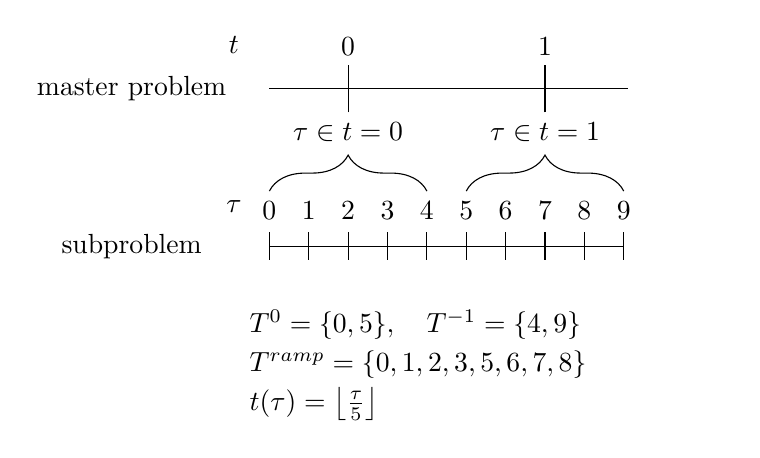
\begin{tikzpicture}
		\node at (0,0) {master problem};
		\draw (1.75,0) -- (6.3,0);
		\node at (1.3,0.55) {$t$};
		\draw (2.75,-0.3) -- (2.75,0.3) node [above] {$0$};
		\draw (5.25,-0.3) -- (5.25,0.3) node [above] {$1$};

		\draw [decorate,decoration={brace,amplitude=13pt}] (1.75,-1.3) -- (3.75,-1.3);
		\draw [decorate,decoration={brace,amplitude=13pt}] (4.25,-1.3) -- (6.25,-1.3);

		\node at (2.75,-0.55) {$\tau \in t = 0$};
		\node at (5.25,-0.55) {$\tau \in t = 1$};

		\node at (0,-2) {subproblem};
		\node at (1.3,-1.5) {$\tau$};
		\foreach \x in {0,1,2,...,9}
		{
		\coordinate (A\x) at ($(1.75,-2)+(\x*0.5cm,0)$) {};
		\draw ($(A\x)+(0,5pt)$) -- ($(A\x)-(0,5pt)$);
		\node at ($(A\x)+(0,3ex)$) {\x};
		}
		\draw (A0) -- (A9);

		\node[text width=6cm] at (4.5, -3) {$T^0 = \{ 0, 5 \}, \quad T^{-1} = \{ 4, 9 \}$};
		\node[text width=6cm] at (4.5, -3.5) {$T^{ramp} = \{ 0, 1, 2, 3, 5, 6, 7, 8 \}$};
		\node[text width=6cm] at (4.5, -4.0) {$t(\tau) = \left \lfloor{\frac{\tau}{5}}\right \rfloor $};
	\end{tikzpicture}
	\caption{$T^0$, $T^{ramp}$, $T^{-1}$, $t(\tau)$, and $\tau \in t$ in an example problem with five subproblem timesteps within each of the two master problem time steps}
	\label{fig_time_scales}
\end{figure}

\section{Solution}

Following \cite{Minguez}, the problem (\ref{saro_obj})-(\ref{master_constraint_last}) is solved using column-and-constraint (CC) algorithm in which solving the first minimization problem of (\ref{saro_obj}) and solving the max-min problem of (\ref{saro_obj}) alternates. These two problems are called CC master problem and CC subproblem, respectively. The alternation terminates when the total costs computed from the two problems match. The formulations for CC master problem and subproblem are given in the following subsections (Eqs. (\ref{cc_master_obj})-(\ref{cc_master_last}) and Eqs. (\ref{sub_obj})-(\ref{sub_last}), respectively) and solution algorithm is described in detail in Algorithm \ref{alg_algorithm}.

\begin{algorithm}
\SetAlgoLined
\DontPrintSemicolon
%\SetKwInOut{Input}{Input}
%\SetKwInOut{Output}{Output}
\textbf{Input:} Transmission and generation parameters, CO\textsubscript{2} emission targets\;
\textbf{Output:} Transmission and generation expansion plan\;
$\epsilon \leftarrow 10^{-6}$ \;
$LB \leftarrow -\infty$ \;
$UB \leftarrow \infty$ \;
$\nu \leftarrow 0$ \;
$d_{o, \tau, n, \nu} \leftarrow \tilde{D}_{o, \tau, n} \quad \forall o, \tau, n$ \;
\While{$(UB - LB) / UB \leq \epsilon$}{
	\tcp*[l]{Solve the CC master problem}
		Obtain \( x_{t, u}^*, \hat{x}_{t, u}^*, \forall t, u \myin \Psi^{G+}; y_{t, \ell}^*, \hat{y}_{t, \ell}^*, \forall t, \ell \myin \Psi^{L+} \) by solving CC master problem in Eqs. (\ref{cc_master_obj})-(\ref{cc_master_last}) using \( d_{o, \tau, n, \nu'}, \forall o, \tau, n, \nu' \leq \nu \). $LB$ is updated to the objective value of the master problem. \;

    \;

	\tcp*[l]{Solve the CC subproblem}
	Obtain \( w_{n} \, \forall n \) by solving CC subproblem in Eqs. (\ref{sub_obj})-(\ref{sub_last}) using the current \( x_{t, u}^*, \forall t, u \myin \Psi^{G+}; y_{t, \ell}^*, \forall t, \ell \myin \Psi^{L+} \). $UB$ is updated to the objective value of the subproblem + $P \sum\limits_{t} R^{-t} \big( \sum\limits_{u \in \Psi^{G+}} C^x_{t, u} \hat{x}_{t, u}^* + \sum\limits_{\ell \in \Psi^{L+}} C^y_{t, \ell} \hat{y}_{t, \ell}^* \big)$ \;

    \;

    $\nu \leftarrow \nu + 1$ \;
    $d_{o, \tau, n, \nu} \leftarrow \tilde{D}_{o, \tau, n} + w_{n} \hat{D}_{o, \tau, n} \quad \forall o, \tau, n$ \;
}
\caption{Algorithm for solving the problem (\ref{saro_obj})-(\ref{master_constraint_last})}
\label{alg_algorithm}
\end{algorithm}

\subsection{CC master problem}

At iteration $\nu$, we have \( \Omega^{M} \myeq \{ g_{o, \tau, u, \nu'}, \forall u; s_{o, \tau, u, \nu'}, \forall u \in \Psi^{G, H}; f_{o, \tau, \ell, \nu'}, \forall \ell; \delta_{o, \tau, n, \nu'}, \forall n \}, \forall o, \tau, \nu' \myleq \nu \). Given \( d_{\tau, n, \nu'}^*, \forall \tau, n, \nu' \myleq \nu \) as input data obtained from all the previous solutions of the subproblem, the master problem at iteration $\nu$ is

\begin{align}
&\label{cc_master_obj} \underset{\Phi^{L1}, \Omega^{M}, \theta}{\text{min}} \, P \sum\limits_{t} R^{-t} \left[ \sum\limits_{u \in \Psi^{G+}} C^x_{t, u} \hat{x}_{t, u} + \sum\limits_{\ell \in \Psi^{L+}} C^y_{t, \ell} \hat{y}_{t, \ell} \right] + \theta \\
&\text{subject to} \nonumber \\
&\text{Eqs. } (\ref{master_constraint_first}) - (\ref{master_constraint_last}) \\
&\label{cc_master_constraint1}\theta \geq \sum\limits_o W_o \sum\limits_{\tau} R^{-t(\tau)} \sum\limits_{u} C_{u}^g g_{o, \tau, u, \nu'} \quad \forall \nu' \leq \nu \\
&\sum\limits_{u | n(u) = n} g_{o, \tau, u, \nu'} - \sum\limits_{\ell | s(\ell) = n} f_{o, \tau, \ell, \nu'} + \nonumber \\
&\sum\limits_{\ell | r(\ell) = n} f_{o, \tau, \ell, \nu'} = d_{\tau, n, \nu'}^* \quad \forall o, \tau, n, \nu' \leq \nu \\
&0 \leq g_{o, \tau, u, \nu'} \leq A_{o, \tau, u} G_{o, \tau, u}^{max} \quad \forall o, \tau, u \in \Psi_n^G, \nu' \leq \nu \\
&0 \leq g_{o, \tau, u, \nu'} \leq A_{o, \tau, u} x_{t(\tau), u} \quad \forall o, \tau, u \in \Psi_n^{G+}, \nu' \leq \nu \\
&G^{ramp,min}_{o, \tau, u} \leq g_{o, \tau + 1, u, \nu'} - g_{o, \tau, u, \nu'} \quad \forall o, \tau \in \Tau^{ramp}, u, \nu' \leq \nu \\
&g_{o, \tau + 1, u, \nu'} - g_{o, \tau, u, \nu'} \leq G^{ramp,max}_{o, \tau, u} \quad \forall o, \tau \in \Tau^{ramp}, u, \nu' \leq \nu \\
&\label{cc_emission_ub}\sum\limits_{o} \sum\limits_{\tau \in t} \sum\limits_{u} W_o G^{emission}_{o, \tau, u} g_{o, \tau, u, \nu'}  \leq E_{t} \quad \forall t, \nu' \leq \nu \\
&s_{o, \tau, u, \nu'} \geq 0 \quad \forall o, \tau, u \in \Psi^{G, H}, \nu' \leq \nu \\
&s_{o, \tau, u, \nu'} = S^0_{o, \tau, u} \quad \forall o, \tau \in \Tau^0, u \in \Psi^{G, H}, \nu' \leq \nu \\
&s_{o, \tau + 1, u, \nu'} = s_{o, \tau, u, \nu'} - g_{o, \tau, u, \nu'} + \nonumber \\
&\quad \quad \quad \quad \quad \, \, \, I_{o, \tau, u} \, \, \forall o, \tau \in \Tau^{ramp}, u \in \Psi^{G, H}, \nu' \leq \nu \\
&S^{min}_{o, \tau, u} \leq s_{o, \tau, u, \nu'} \leq S^{max}_{o, \tau, u} \quad \forall o, \tau \in \Tau^{-1}, u \in \Psi^{G, H}, \nu' \leq \nu \\
&f_{o, \tau, \ell, \nu'} = B_\ell (\delta_{o, \tau, s(\ell), \nu'} - \delta_{o, \tau, r(\ell), \nu'}) \quad \forall o, \tau, \ell \in \Psi^L, \nu' \leq \nu \\
&\label{cc_master_constraint_benders1}F_{o, \tau, \ell}^{min} \leq f_{o, \tau, \ell, \nu'} \leq F_{o, \tau, \ell}^{max} \quad \forall o, \tau, \ell \in \Psi^L, \nu' \leq \nu \\
&F_{o, \tau, \ell}^{min} y_{t(\tau), \ell} \leq f_{o, \tau, \ell, \nu'} \leq F_{o, \tau, \ell}^{max} y_{t(\tau), \ell} \, \forall o, \tau, \ell \in \Psi^{L+}, \nu' \leq \nu \\
&\label{cc_master_constraint_benders2}-\pi \leq \delta_{o, \tau, n, \nu'} \leq \pi \quad \forall o, \tau, n, \nu' \leq \nu \\
&\label{cc_master_last} \delta_{o, \tau, 0, \nu'} = 0 \quad \forall o, \tau, \nu' \leq \nu
\end{align}

\subsection{CC subproblem}

For the subproblem, we set
\begin{align*}
\Omega^{S} = &\{ \bar{\beta}_{o, \tau, u}, \underline{\beta}_{o, \tau, u}, \bar{\beta}_{o, \tau, u}^{ramp}, \underline{\beta}_{o, \tau, u}^{ramp} \}, \forall o, \tau, u \; \cup \\
&\beta_{t}^{emission}, \forall t \; \cup \\
&\{ \phi_{o, \tau, u}^{0}, \forall \tau \myin \Tau^0; \phi_{o, \tau, u}, \forall \tau \myin \Tau^{ramp}; \\
&\, \, \, \bar{\phi}_{o, \tau, u}^{-1}, \underline{\phi}_{o, \tau, u}^{-1} \forall \tau \myin \Tau^{-1}; \underline{\phi}_{o, \tau, u} \forall \tau \}, \forall o, u \myin \Psi^{G, H} \; \cup \\
&\{ \mu_{o, \tau, \ell}, \bar{\mu}_{o, \tau, \ell}, \underline{\mu}_{o, \tau, \ell} \} \forall o, \tau, \ell \; \cup \\
&\{ \lambda_{o, \tau, n}, \bar{\mu}^{va}_{o, \tau, n}, \underline{\mu}^{va}_{o, \tau, n} \}, \forall o, \tau, n \; \cup \\
&\mu^{ref}_{o, \tau}, \forall o, \tau.
\end{align*}
%\(  \myeq \{ \bar{\beta}_{o, \tau, u}, \underline{\beta}_{o, \tau, u}, \bar{\beta}_{o, \tau, u}^{ramp}, \underline{\beta}_{o, \tau, u}^{ramp} \}, \forall o, \tau, u \mycup \beta_{t}^{emission}, \forall t \mycup \)
%\( \{ \phi_{o, \tau, u}^{0}, \forall \tau \myin \Tau^0; \phi_{o, \tau, u}, \forall \tau \myin \Tau^{ramp}; \)
%\( \bar{\phi}_{o, \tau, u}^{-1}, \underline{\phi}_{o, \tau, u}^{-1} \forall \tau \myin \Tau^{-1}; \underline{\phi}_{o, \tau, u} \forall \tau \}, \forall o, u \myin \Psi^{G, H} \mycup \)
%\( \{ \mu_{o, \tau, \ell}, \bar{\mu}_{o, \tau, \ell}, \underline{\mu}_{o, \tau, \ell} \} \forall o, \tau, \ell \mycup \)
%\( \{ \lambda_{o, \tau, n}, \bar{\mu}^{va}_{o, \tau, n}, \underline{\mu}^{va}_{o, \tau, n} \}, \forall o, \tau, n \mycup \mu^{ref}_{o, \tau}, \forall o, \tau \)
With $x_{t, u}^*, \forall t, u \myin \Psi^{G+}$ and $y_{t, \ell}^*, \forall t, \ell \myin \Psi^{L+}$ as input data obtained from the previous solution of the master problem, the subproblem is
\begin{align}
\label{sub_obj} \underset{\Phi^{L2}, \Omega^{S}}{\text{maximize}} &\sum\limits_o \Bigg( \sum\limits_{\tau} \Big[ \sum\limits_n \lambda_{o, \tau, n} d_{o, \tau, n} - \nonumber \\
&\sum\limits_{u \in \Psi^G} \bar{\beta}_{o, \tau, u} A_{o, \tau, u} G_{o, \tau, u}^{max} - \nonumber \\
&\sum\limits_{u \in \Psi^{G+}} \bar{\beta}_{o, \tau, u} A_{o, \tau, u} x_{t(\tau), u}^* - \nonumber \\
&\sum\limits_{\ell \in \Psi^L} \left( \bar{\mu}_{o, \tau, \ell} F_{o, \tau, \ell}^{max} - \underline{\mu}_{o, \tau, \ell} F_{o, \tau, \ell}^{min} \right) - \nonumber \\
&\sum\limits_{\ell \in \Psi^{L+}} \left( \bar{\mu}_{o, \tau, \ell} F_{o, \tau, \ell}^{max} - \underline{\mu}_{o, \tau, \ell} F_{o, \tau, \ell}^{min} \right) y_{t(\tau), \ell}^* - \nonumber \\
&\sum\limits_{n} \pi ( \bar{\mu}^{va}_{o, \tau, n} + \underline{\mu}^{va}_{o, \tau, n} ) \Big] + \nonumber \\
&\sum\limits_{u \in \Psi^{G, H}} \Big[ \sum\limits_{\tau \in \Tau^{0}}  \phi_{o, \tau, u}^{0} S^{0}_{o, \tau, u} + \nonumber \\
&\sum\limits_{\tau \in \Tau^{ramp}} \phi_{o, \tau, u} I_{o, \tau, u} + \nonumber \\
&\sum\limits_{\tau \in \Tau^{-1}} \left( \underline{\phi}^{-1}_{o, \tau, u} S^{min}_{o, \tau, u} - \bar{\phi}^{-1}_{o, \tau, u} S^{max}_{o, \tau, u} \right) \Big] + \nonumber \\
&\sum\limits_{\tau \in \Tau^{ramp}} \sum\limits_{u} \left( \underline{\beta}_{o, \tau, u}^{ramp} G^{ramp,min}_{o, \tau, u} - \bar{\beta}_{o, \tau, u}^{ramp} G^{ramp,max}_{o, \tau, u} \right) \Bigg) - \nonumber \\
&\sum\limits_{t} \beta_{t}^{emission} E_{t}
\end{align}
\begin{align}
&\text{subject to} \nonumber \\
&\lambda_{o, \tau, n(u)} - \bar{\beta}_{o, \tau, u} + \underline{\beta}_{o, \tau, u} + \mathbbm{1}_{\tau \in \Tau^{ramp} \land u \in \Psi^{G, H}} \phi_{o, t, u} - \nonumber \\
&\mathbbm{1}_{\tau \notin \Tau^0} \bar{\beta}_{o, \tau - 1, u}^{ramp} + \mathbbm{1}_{\tau \notin \Tau^{-1}} \bar{\beta}_{o, \tau, u}^{ramp} + \mathbbm{1}_{\tau \notin \Tau^0} \underline{\beta}_{o, \tau - 1, u}^{ramp} - \nonumber \\
&\label{sub_constr1}\mathbbm{1}_{\tau \notin \Tau^{-1}} \underline{\beta}_{o, \tau, u}^{ramp} - W_o G_{u}^{emission} \beta_{t(\tau)}^{emission} {=} R^{-t(\tau)} C^g_{u}  W_o \; \forall o, \tau, u \\
&\mathbbm{1}_{\tau \in \Tau^0} \phi_{o, \tau, u}^{0} + \underline{\beta}_{o, \tau, u}^s - \mathbbm{1}_{\tau \notin \Tau^{-1}} \phi_{o, \tau, u} + \mathbbm{1}_{\tau \notin \Tau^0} \phi_{o, \tau - 1, u} + \nonumber \\
&\mathbbm{1}_{\tau \in \Tau^{-1}} (\underline{\phi}_{o, \tau, u} - \bar{\phi}_{o, \tau, u}) = 0 \quad \forall o, \tau, u \in \Psi^{G, H} \\
&-\lambda_{o, \tau, s(\ell)} + \lambda_{o, \tau, r(\ell)} + \mathbbm{1}_{\ell \in \Psi^{L,AC}} \mu_{o, \tau, \ell} - \nonumber \\
&\bar{\mu}_{o, \tau, \ell} + \underline{\mu}_{o, \tau, \ell} = 0 \quad \forall o, \tau, \ell \\
&-\sum\limits_{\ell \in \Psi^{L,AC} | s(\ell) = n} B_\ell \mu_{o, \tau, \ell} + \sum\limits_{\ell \in \Psi^{L,AC} | r(\ell) = n} B_\ell \mu_{o, \tau, \ell} - \nonumber \\
&\bar{\mu}^{va}_{o, \tau, n} + \underline{\mu}^{va}_{o, \tau, n} + \mathbbm{1}_{n = 0} \mu^{ref}_{o, \tau} = 0 \quad \forall o, \tau, n \\
&\label{sub_last}\text{Eqs. } (\ref{uncertainty_set1})-(\ref{uncertainty_set2}),
\end{align}
where $\mathbbm{1}_{cond}$ equals 1 if $cond$ is true and otherwise 0.

The subproblem can be solved directly as a MIQP using solvers such as Gurobi. Alternatively, the subproblem can be re-formulated as an MILP by linearizing the product of a continuous and a binary variable in $\lambda_{o, \tau, n} d_{o, \tau, n} = \lambda_{o, \tau, n} D^{-t(\tau)} (\tilde{D}_{o, \tau, n} + w_n \hat{D}_{o, \tau, n})$ in the objective function (\ref{sub_obj}) exactly with $\lambda_{o, \tau, n} d_{o, \tau, n} = D^{-t(\tau)} (z_{o, \tau, n} \hat{D}_{o, \tau, n} + \lambda_{o, \tau, n} \tilde{D}_{o, \tau, n})$ and by adding the following constraints to the subproblem
\begin{align}
&\label{z_constr} z_{o, \tau, n} = \lambda_{o, \tau, n} - \tilde{\lambda}_{o, \tau, n} \quad \forall o, \tau, n \\
&\Lambda^{min} w_n \leq z_{o, \tau, n} \leq \Lambda^{max} w_n \quad \forall o, \tau, n \\
&\Lambda^{min} (1 - w_n) \leq \tilde{\lambda}_{o, \tau, n} \leq \Lambda^{max} (1 - w_n) \quad \forall o, \tau, n,
\end{align}
where parameters $\Lambda^{min}$ and $\Lambda^{max}$ can be set to exchange-specific values such as -500 €/MWh and 3000 €/MWh, respectively.

\subsection{Benders decomposition of the CC master problem}

The CC master problem in Eqs. (\ref{cc_master_obj})-(\ref{cc_master_last}) is an MILP that grows in the number of constraints at every CC iteration $\nu$ whereas the CC subproblem remains fixed in size. If multiple iterations are required for solving a medium to large problem instance (i.e. several nodes, generation units, transmission lines and time steps), then the CC master problem can become prohibitively expensive. To tackle this issue, we apply Benders decomposition to the CC master problem to convert it to a small MILP and a large LP that are solved alternatively. Even though these two problems grow also at every CC iteration, they are typically faster to solve than the original MILP as we later see in Section \ref{section_case_study}.

More specifically, the complicating variables in the original CC master problem are the binary variables $y_{t, \ell}$ and $\hat{y}_{t, \ell}$ that, once fixed, render an LP problem. Thus, the Benders master problem at iteration $k$ chooses $\Phi^{L1, BM} = \{ y_{t, \ell}, \hat{y}_{t, \ell}, \forall t, \ell \in \Psi^{L+} \}$ by solving the following problem given $(blaa)$ ...

\begin{align}
&\label{benders_master_obj} \underset{\Phi^{L1, BM}, \eta}{\text{min}} \, P \sum\limits_{t} R^{-t} \sum\limits_{\ell \in \Psi^{L+}} C^y_{t, \ell} \hat{y}_{t, \ell} + \eta \\
&\text{subject to} \nonumber \\
&\eta - \sum\limit_{o} \sum\limit_{\tau} \sum\limit_{\nu} \Bigg[ \sum\limits_{u \in \Psi^G} \Big( A_{o, \tau, u} G_{o, \tau, u}^{max} \bar{\beta}_{o, \tau, u, \nu} + \nonumber \\
&\mathbbm{1}_{\tau \in \Tau^{ramp}} (G^{ramp,max}_{o, \tau, u} \bar{\beta}_{o, \tau, u, \nu}^{ramp} - G^{ramp,min}_{o, \tau, u} \underline{\beta}_{o, \tau, u, \nu}^{ramp}) \Big) + \nonumber \\
&\sum\limit_{\ell \in \Psi^{L+}} y_{t(\tau), \ell} (F_{o, \tau, \ell}^{max} \bar{\mu}_{o, \tau, \ell, \nu} - F_{o, \tau, \ell}^{min} \underline{\mu}_{o, \tau, \ell, \nu}) + \nonumber \\
&\sum\limit_n d_{o, \tau, n, \nu}^* \sigma_{o, \tau, n, \nu} + \sum\limit_n \pi (\bar{\mu}^{va}_{o, \tau, n, \nu} + \underline{\mu}^{va}_{o, \tau, n, \nu}) + \nonumber \\
&\sum\limit_{u \in \Psi^{G,H}} \Big( \mathbbm{1}_{\tau \in \Tau^{0}} S^0_{o, \tau, u} \phi_{o, \tau, u, \nu}^{0} + \mathbbm{1}_{\tau \in \Tau^{ramp}} I_{o, \tau, u} \phi_{o, \tau, u, \nu} + \nonumber \\
&\mathbbm{1}_{\tau \in \Tau^{-1}} (S^{max}_{o, \tau, u} \bar{\phi}_{o, \tau, u, \nu} - S^{min}_{o, \tau, u} \underline{\phi}_{o, \tau, u, \nu}) \Big) \Bigg] - \nonumber \\
&\sum\limit_{t} \sum\limit_{\nu} E_{t} \beta_{t}^{emission} \geq 0
\end{align}

With $y^*_{t, \ell, k}$ and $\hat{y}^*_{t, \ell, k}$ as input data, the Benders subproblem at iteration $k$ is then given by $\Phi^{L1, BS} = \{ x_{t, u}, \hat{x}_{t, u}, \forall t, \ell \in \Psi^{G+} \}$
\begin{align}
&\label{benders_sub_obj} \underset{\Phi^{L1}, \Omega^{M}, \theta}{\text{min}} \, P \sum\limits_{t} R^{-t} \left[ \sum\limits_{u \in \Psi^{G+}} C^x_{t, u} \hat{x}_{t, u} + \sum\limits_{\ell \in \Psi^{L+}} C^y_{t, \ell} \hat{y}^*_{t, \ell} \right] + \theta \\
&\text{subject to} \nonumber \\
&\textrm{1st level constraints (\ref{master_constraint_first}) and (\ref{master_constraint_last})} \nonumber \\
&\textrm{3rd level constraints (\ref{cc_master_constraint1})-(\ref{cc_master_constraint_benders1}), (\ref{cc_master_constraint_benders2}), and (\ref{cc_master_last}}) \nonumber \\
&F_{o, \tau, \ell}^{min} y^*_{t(\tau), \ell, k} \leq f_{o, \tau, \ell, \nu'} \leq F_{o, \tau, \ell}^{max} y^*_{t(\tau), \ell, k} \, \forall o, \tau, \ell \in \Psi^{L+}, \nu' \leq \nu
\end{align}

%Note that the above Benders subproblem may be parallelizable across operating conditions $o$ or time steps $t$ or $\tau$ for some problem formulations. However, in our model, the constraints (\ref{master_constraint_first}) and (\ref{cc_emission_ub}) prevent parallelization.

\section{Case study: 10-year investment plan for modified Nordic and Baltic network}
\label{section_case_study}

\subsection{Data}

We study what investments are required to decrease the initial \COtwo emissions of the Nordic and Baltic electricity system to a target level under uncertain generation and transmission parameters and worst-case realization of demand. More specifically, we use the Nordic and Baltic network and its generation, load, and transmission line data from \cite{Virasjoki} as a base.

We augment this base system by having 10 time steps in the CC master problem ($t$) for making investments. For each master problem time step, we consider 24 time steps in the CC subproblem ($\tau$). Consequently, the subproblem has 240 time steps in total. To consider increasing electricity demand, we assume that load values increase by a factor of $D = 1.01$ at each master problem time step \cite{EEA_consumption}.

In addition, we define 3 operation conditions $o$ for each subproblem time step. We apply the hierarchical clustering method of \cite{Nahmmacher} on hourly load and wind power data of 2014 to obtain 3 representative days. The hourly load, wind, and solar power data on these 3 representative days are used as the operating conditions for each set of 24 subproblem time steps. This allows us to capture the short-term variability of load and renewables. Hydro power data such as initial storage levels ($S_{o, \tau, u}^0$) and inflows ($I_{o, \tau, u}$) have weekly granularity so, for each operating condition, we take the weekly value corresponding to each representative day. However, for generation ($G^{max}_{o, \tau, u}$) and transmission capacities ($F^{max}_{o, \tau, \ell}$ and $F^{min}_{o, \tau, \ell}$), the operation conditions are defined by sampling uniform noise from $\textrm{U}(-50 \textrm{ MW}, 50 \textrm{ MW})$. The weights of the operation conditions ($W_o$) are equal to the weights of the representative days as defined in \cite{Nahmmacher}.

Gas, CCGT, oil, biomass, wind and solar power can be built at each (non-dummy) node. Each candidate unit has a maximum capacity ($G^{inv,max}_u$) of 10000 MW except for biomass units which we limit to 1000 MW due to limited fuel supply. In addition, neighboring (non-dummy) node pairs can be connected with a candidate DC transmission line with 1000 MW of capacity to both directions. The investment cost parameters are shown in Table \ref{table_investment_parameters}.

The initial \COtwo emission bound $E_{0} = 90000 \textrm{ tonne}$ is obtained from the \COtwo emissions corresponding to the first master problem time step when solving the problem with no investments. This initial emission bound is realistic given that the average daily \COtwo emissions of both power and heat production were approximately $E_{0} = 140000 \textrm{ tonne}$ in this area in 2014 \cite{EEA_COtwo}. We assume that the \COtwo emissions are required to decrease by approximately 10\% at every master problem time step to a final emission bound of $E_{9} = 35000 \textrm{ tonne}$.

The uncertainty budget in the subproblem ($\Lambda^w$) is 2 meaning that the model can change load in maximum of 2 nodes. Each change the model makes increases load in a node for all operating conditions and subproblem time steps by $\hat{D}_{\tau, n} = 100 \textrm{ MWh}$.

\begin{table}[htpb]
\centering
\begin{tabular}{l| c} \hline
Parameter 					& Value  \\ \hline
$P$ 						& $\frac{1}{365}$ \\
$R$							& 1.03		\\
$C^x_{0, u}$ Gas (€/MW)		& 0.8 \cdot 10^6    \\
$C^x_{0, u}$ CCGT (€/MW)	& 1.0 \cdot 10^6    \\
$C^x_{0, u}$ Oil (€/MW)		& 0.8 \cdot 10^6    \\
$C^x_{0, u}$ Biomass (€/MW)	& 3.9 \cdot 10^6    \\
$C^x_{0, u}$ Wind (€/MW)	& 1.6 \cdot 10^6    \\
$C^x_{0, u}$ Solar (€/MW)	& 1.8 \cdot 10^6    \\
$C^y_{0, \ell}$ (€)			& 1.0 \cdot 10^9	\\
\end{tabular}
\caption{Investment cost parameters in the case study}
\label{table_investment_parameters}
\end{table}

\subsection{Results}

We solve this case study using the Algorithm \ref{alg_algorithm} such that, for the CC master problem, we consider MILP and Benders decomposition formulations and, for the CC subproblem, we consider MILP and MIQP formulations. The results in Table \ref{table_results} show that all formulations attain the same objective value while the combination of Benders decomposition and MIQP is the fastest. The majority of time is spent at solving the last CC master problem so changing the CC subproblem formulation provides only a limited benefit.

\begin{table}[htpb]
\centering
\begin{tabular}{c c| c c c} \hline
Master problem 			& Subproblem 		& Objective value (€) 	& Solution time (s) & Iterations \\ \hline
Benders					& MIQP 				& 95915334.5162 		& 856.0				& 3				 \\
MILP					& MIQP 				& 95915334.5162 		& 1656.18			& 3				 \\
\end{tabular}
\caption{}
\label{table_results}
\end{table}

Figure \ref{fig_emissions} shows the evolution of \COtwo emissions to the final desired level during the planning horizon and the corresponding \COtwo emission prices. Figures \ref{fig_generation_investment} and \ref{fig_transmission_investment} show the generation and transmission investments, respectively, for achieving the final emission level. Already at $t = 0$, the model builds transmission lines from Finland to Norway and Sweden and a total of 1600 MW of CCGT units in Latvia and Lithuania as well as 1100 MW of wind power in Finland. As a consequence, \COtwo emissions from $t = 0$ to $t = 4$ are below the bounds until demand increases to a high enough level at $t = 5$. To reduce \COtwo emissions to the final level, the model invests in approximately 700 MW of biomass units in Estonia.

The generation mixes in Figure \ref{fig_generation_mixes} show that, compared to a solution with minimal investments and no emission constraint, the above transmission and generation investments allow replacing coal-, oil, and oil shale-fired generation with less-polluting wind power as well as gas and biomass-fired generation. In addition, new transmission lines between Finland, Norway, and Sweden enable increased levels of hydro power and nuclear generation until their maximum capacity is achieved.

\begin{figure}[htpb]
  \centering
  \includegraphics[width=\linewidth]{emissions_milp_dc_miqp_dc.png}
  \caption{\COtwo emissions and prices during the planning horizon}
  \label{fig_emissions}
\end{figure}

\begin{figure}[htpb]
	\centering
	\includegraphics[width=\linewidth]{generation_investment_milp_dc_miqp_dc.png}
	\caption{Generation investments during the planning horizon. The country codes indicate the node where each generation unit is built}
	\label{fig_generation_investment}
\end{figure}

\begin{figure}[htpb]
	\centering
	\includegraphics[width=\linewidth]{transmission_investment_milp_dc_miqp_dc.png}
	\caption{Transmission investments during the planning horizon. The country codes indicate the start and end node of each line}
	\label{fig_transmission_investment}
\end{figure}

\begin{figure}[htpb]
	\centering
	\includegraphics[width=\linewidth]{generation_mixes.png}
	\caption{Generation mixes with a model without and with an emission constraint}
	\label{fig_generation_mixes}
\end{figure}

\subsection{Cost of robustness}

Next, we evaluate the out-of-sample performance of the SARO model under different load levels. As a comparison, we use stochastic programming (SP) model in which the uncertainty budget of $\Lambda^w = 2$ for load increases of $\hat{D}_{\tau, n} = 100 \textrm{ MWh}$ is randomly allocated to the nodes. Figure \ref{fig_cost_of_robustness} indicates that the SARO model is more conservative in that it has higher total costs when load change is zero or negative. However, for positive load changes, the SARO model has lower total costs than the SP model.

\begin{figure}[htpb]
	\centering
	\includegraphics[width=\linewidth]{cost_of_robustness.png}
	\caption{Performance of different models under different load levels}
	\label{fig_cost_of_robustness}
\end{figure}

\section{Conclusions}
\label{section_conclusions}

This paper proposes a SARO model for the G\&TEP problem with multiple time periods and with a emission reduction goal. In addition, we propose Benders decomposition and MIQP reformulations to solving the problem. We apply the model to a Nordic and Baltic power system and make the following conclusions:

\begin{enumerate}
	\item New transmission line investments are built to make flexible and environmentally-friendly hydro power production available in the entire system.
	\item New wind power units are built to reduce emissions. In addition, CCGT and biomass generation units are built to displace more polluting coal and oil-shale units and to provide flexibility for offsetting the variability of wind and solar power.
	\item The solution found by the SARO model outperforms that of a stochastic programming model on higher load levels but is more expensive on lower load levels.
	\item Benders decomposition speeds up the solution of a large and growing MILP by splitting it up to a small MILP and a large LP.
	\item MIQP formulation speeds up the solution of the subproblem.
\end{enumerate}

Future work could explore longer-term investment plans with various scenarios on the electrification of transportation as well as deployment of emerging technologies such as storage. Moreover, the model could be extended to cover larger power systems such as the entire Europe to find a more globally optimal investment plan that takes into account the pool of resources and spatio-temporal correlations of VRES generation in a larger geographical area. Also, considering additional sources of uncertainty such as transmission and generation outages could lead to more robust investment plans for renewable-rich systems. Finally, the growing large LP in the Benders subproblem remains a bottleneck so exploring the possibilities to further decompose it could lead to significant improvements in solution times.

\bibliographystyle{IEEEtran}
\bibliography{IEEEabrv,references}


\end{document}